\chapter{Proposal}
\label{chapter-proposal}
In this chapter, we will present our proposal to realize general and autonomous artificial researcher.

% discuss what should be done and how to achieve the realization of autonomous artificial researchers. Firstly, we will provide an overview of Chapter 1 and Chapter 2. Building upon that, we will propose sub-goals to aim for in order to achieve autonomous artificial researchers. Subsequently, for each sub-goal, we will organize subtasks and propose a general approach and strategy for how to pursue these intermediate goals.

% As we have reiterated multiple times, the ultimate goal is to create an artificial intelligence that can autonomously conduct research. Therefore, in order to clarify the objectives, it is necessary to define what it means for an AI to be able to conduct research and what it means for it to be autonomous. Let's first discuss these aspects. 

\section{Constructing a Research Pipeline}
We propose to start by building a research pipeline, connecting the modules of the knowledge production system. The research pipeline is a software system that takes input and generates knowledge as output, encompassing the sequence of processes involved in research. Since this process does not require human intervention, it can be considered as an autonomous research system. We propose this system to be composed of the sub-processes of ``question construction,'' ``hypothesis generation,'' and ``hypothesis verification.'' This creates a general system that is potentially applicable to any research. These sub-processes can be likened to abstract classes in programming. Each process automatically formulates appropriate questions, generates hypotheses, and performs verification based on the input. 

Initially, we will assume a specific research problem, and this research problem can be a simple one. And the inner workings of detailed hypothesis testing and hypothesis generation can be guided (but not hard-coded) to achieve the desired results. Anyway, the high-level concept is to create the minimum necessary to automatically execute each process of question construction, hypothesis generation, and hypothesis testing. Then, by gradually making the contents of each module autonomous and gradually loosening the restrictions on the research problem, we will lead to a general-purpose and autonomous artificial researcher.

\subsubsection{Guided but Not Hard-Coded}

It is important to note, however, that even in the prototype stage, the internal implementation of question construction, hypothesis generation, hypothesis testing, etc., should be ``guided'' and not ``hard-coded'' as much as possible. In machine learning, induction is the process of adding words to the prompt that make it easier to output the expected answer, and hardcoding is the process of actually inserting the desired processing into the algorithm. For example, if a statistical hypothesis test is expected to be used as a means of testing a hypothesis, rather than having a human write a program that contains a process for performing a statistical hypothesis test, we would instead instruct to the machine learning model with prompting, ``Statistical hypothesis testing is one of the leading methods in verification. The hypothesis is A. Verify this.'' This is a very important point to emphasize.

This is a very important point, so let me emphasize it. The reason this is important is that we do not want to automate a particular hypothesis testing process, but rather we want the machine to test the hypothesis itself. Only when you make sure that the machine decides on its own the appropriate verification method according to the hypothesis, will you be able to provide collateral evidence that the machine itself is able to verify the hypothesis. If this can be done not only in hypothesis testing, but also in all aspects of question construction and hypothesis generation, we can call it a prototype of a general-purpose, autonomous artificial researcher.

\subsubsection{Why Pipeline?}

There are two reasons why we think it is a good idea to start by building such a research process pipeline. The first is that this is one simplified representation of a generic and autonomous research system. Research is a very complex task, so when we try to automate validation, we inevitably focus on automating individual tasks. In addition, many research automation efforts are aimed at making things better, which often leads to a strong dependence on the domain, for example, in automating hypothesis generation. However, as emphasized above, what we want to achieve is not specific hypothesis generation or verification, but the ability to generate and verify hypotheses themselves. This system emphasizes that point, and once realized, it will be an example of what a general-purpose, autonomous artificial researcher could look like. The creation of such an example will serve as a guidepost for more people to become versatile and autonomous artificial researchers.

Second, building on this would further clarify the challenges in achieving a general-purpose and autonomous artificial researcher. In this paper, we have discussed the challenges that would be necessary to realize a general-purpose, autonomous artificial researcher. However, we believe that this is a very difficult task and that there are many areas where we do not even know what the problems really are. Therefore, it is important to first identify what the problems are in the first place and where the uncertainties lie. When we move toward such a complex problem, we start with a simple example to understand the structure of the problem. For example, we build toy models in physics, concrete examples in mathematics, and prototypes in programming. The research process pipeline falls under such simple examples in autonomous artificial researchers. In the process of trying to achieve this, we will discover what are the bottlenecks and what are the essentials. In this way, I think it is important to build a research process pipeline in order to first increase the resolution of the problem and clarify the issues.

\subsubsection{Where to Start?}
It is advisable to start by representing a specific research as a pipeline. Initially, creating a concrete system helps clarify the actions involved in actual research and makes the specific challenges to be addressed more tangible. When dealing with projects with high uncertainty, it is crucial to concretize the problems to be solved. Specifically, the goal is to programmatically represent the actions that researchers perform as comprehensively as possible. It is acceptable to consider certain aspects as constants if their execution is too challenging to represent as a program. Then, running the system should reproduce the original research. The next step is to progressively automate the processes and constants provided by humans to enhance autonomy. Naturally, automating a specific research pipeline alone does not guarantee the development of an autonomous pipeline. However, this approach allows for the identification of research automation challenges and paves the way for their resolution through research and development. Importantly, it is essential to express individual tasks as components or sub-processes of question construction, hypothesis generation, or hypothesis verification. This is similar to inheriting an abstract class, ensuring that the automation of these processes is achieved as individual tasks are automated.

In practice, it becomes evident that fully automating an entire research is highly challenging. Therefore, before automating specific research, it may be advantageous to start by creating simplified toy models and aiming to build systems that can execute them automatically. For example, certain parts that require obtaining and using a real dataset can be replaced with appropriately created sample datasets. The approach is similar to that of specific research pipelines, addressing research challenges while aiming to increase autonomy and generality.

\textcolor{red}{Remarks about Autores PJ}

\section{Where to Start}

Research in the field of machine learning is suitable as a specific research to start with. Firstly, many machine learning studies are conducted entirely on computers. As mentioned earlier, the greatest difficulty in achieving universal automation lies in the interaction with the real world. Technologies related to real-world interaction are used for hypothesis verification rather than the verification itself. This requires advancements in robotics research. Therefore, to pursue the automation of the entire research process, it may be best to set aside fields that require interaction with the real world and initially focus on automating research that can be done solely on PCs. Secondly, many attempts to automate machine learning processes have already been made. For example, in MLOps, various pipelines for automating tasks such as experiment management and training in machine learning have been proposed and put into practical use. AutoML, which is a field of machine learning research, has also produced numerous innovations in automating many of the tasks involved in machine learning. Moreover, the culture of machine learning and related engineering fields already has a wealth of knowledge and insights regarding automation. By effectively utilizing this knowledge, it may be possible to achieve research pipeline realization more efficiently compared to other fields. Thirdly, machine learning researchers and engineers who undertake research automation are likely to be more familiar with machine learning research. Fourthly, many studies in machine learning and related research areas are open-source. Consequently, it is considered easier to retrieve information from papers compared to other fields. For these reasons, I believe it is a good approach to start by automating a specific research project in the machine learning domain.

\section{Bootstrapping}
Do research automation that contribute to research automation research.

\section{Others}
When classifying efforts in research automation based on two axes: generality and autonomy, they can be categorized as follows:

% To reiterate, the proposition put forward in this paper is to strive for the realization of autonomous intelligent systems that can conduct research. This is because I believe it holds the potential to liberate research from the cognitive, historical, and social constraints that surround humans. Furthermore, I think it can lead to a future where better knowledge production occurs, ultimately enabling a broader and deeper understanding of the universe and nature.

% I believe that more people should engage in efforts aimed at developing artificial intelligence that autonomously conducts research on universal subjects. This is because there currently seems to be a limited number of such endeavors. Firstly, I think efforts in research automation can be classified along the axes of universality and autonomy. Universality refers to how many research fields a single automated research system can handle. For example, a system capable of conducting research in both physics and history would have higher universality compared to a system limited to either one. This can be understood as the ability to tackle universal questions. Next, autonomy refers to the level of human intervention involved. For instance, a system that requires humans to explicitly provide a set of hypotheses has lower autonomy compared to one that allows the machine to discover them on its own. From this perspective, previous endeavors in research automation can be organized as illustrated in the following diagram. (Diagram description). Thus, it can be said that there are still relatively few efforts focused on constructing highly universal and autonomous automated research systems.

\textcolor{red}{TODO: Add Fig}

% Of course, efforts to automate research at all levels are important. For example, initiatives to automate a specific experiment in physics are valuable in their own right, as they aim to achieve the specific objective of enabling more efficient research. Therefore, the endeavors mentioned in this paper differ in their original goals, and it is not a matter of determining which is better or more important. Additionally, insights gained from these endeavors related to the construction of highly universal and autonomous systems are crucial. As achieving such systems involves high uncertainty, it is beneficial to start by creating concrete systems to increase problem resolution. This process will involve considering which aspects of a specific system can be abstracted to achieve universality and autonomy. Hence, the most important aspect is that all initiatives aspiring towards research automation gain momentum.

% \subsection{Goal and Research}
% First, let's discuss what it means for an AI to be able to conduct research. We delved into this topic in detail in Chapter 2. Research is the act of producing new knowledge for a community of constituents capable of forming shared beliefs. Producing new knowledge involves posing unanswered questions, formulating hypotheses in response to those questions, and verifying those hypotheses to update beliefs. Therefore, creating an intelligent system capable of conducting research means creating a system that can perform these tasks.

% \textcolor{red}{TODO: revision}

% \subsection{Goal and Autonomy}
% The ultimate goal is to create an artificial intelligence that can produce knowledge. In other words, the aim is to develop a function that can autonomously generate some form of knowledge when given any input. Therefore, any attempt to achieve the realization of an artificial researcher should strive to create such a function, regardless of its specific form. As we have reiterated, if the knowledge generated through research is a shared belief in a justified and true society, then the goal can be rephrased as aiming to generate a belief in response to any input and justify it to the extent that it becomes a shared belief in a society.

\textcolor{red}{TODO: revision}

% \section{What to Do to Achieve the Objective}

% To create a universal artificial researcher, I believe it is necessary to automate the construction of questions, generation of hypotheses, and verification of hypotheses. This is because, as seen in Chapter 1, these functions appear to be essential in all research. In other words, by automating these functions as much as possible without relying on human intervention, we can move closer to the realization of an autonomous and universal artificial researcher.

% \subsection{question construction}
% The construction of a question is the act of seeking information \cite{watson2015ask}. Specifically, in the context of research, we consider information as knowledge. The act of seeking knowledge involves two steps: 1. Recognizing the lack of knowledge and 2. Attempting to fill that knowledge gap. In this discussion, we assume that intelligence is designed to consistently generate questions when given input. Therefore, we temporarily set aside the aspect of "triggering action" related to the second step of attempting to fill the knowledge gap.

% The recognition of a knowledge gap occurs when we expect to have certain knowledge and, upon referencing our accessible knowledge, we find that it is not available. For example, when running a program and encountering an error that we cannot resolve on our own, we recognize that we lack the necessary knowledge.

% The reasons for expecting the existence of certain knowledge can vary and are arbitrary. In this case, we assume that a purpose given by a third party creates an expectation of certain knowledge. For example, in the case of humans, we first consider what we need to do to achieve a certain purpose. We then anticipate the necessary knowledge to accomplish those tasks, and when we find that it is not present within our existing knowledge, we recognize the knowledge gap.

% Lastly, in this discussion, knowledge refers to the collective body of research findings, particularly academic papers. In actual research, a researcher may personally have a question and then investigate previous studies to confirm that it is indeed unknown before formulating it as a research question. However, what is important in the construction of a research question is that it is unknown to other entities. Therefore, for simplicity, we directly refer to the entirety of academic papers without including the step of comparing personal knowledge.

% To summarize, to create an intelligence capable of constructing questions in this setting, we need to design it to expect the necessary knowledge to achieve a given purpose provided by a third party, search for that knowledge in academic papers, assess whether the papers contain sufficient knowledge to achieve the purpose, and express any knowledge gaps as questions.

% In this case, we excluded the discussion of triggering action by design. However, when considering increasing autonomy, it is important to discuss how to incorporate this aspect into learning and acquisition. The question of "why do we seek information" has been extensively discussed in the context of curiosity.

% Furthermore, in this case, we defined the expectation of knowledge as aiming to achieve a given purpose. However, as mentioned earlier, this does not affect the formulation of questions. For example, let's consider the case of a child asking, ``Why is the sky blue?'' In this case, the child may already have prior knowledge of the concept of ``sky'' and ``blue.'' Additionally, they may possess a naive concept of causality, believing that ``A is B, so there must be a reason for it.'' Thus, they may have expected to have the knowledge that ``the sky is blue because of B.'' However, when they reference their internal knowledge, they find that it does not contain the corresponding knowledge. Therefore, they may have asked the question ``Why is the sky blue?'' to evoke the knowledge they were lacking.

% In this way, the reasons for expecting the existence of certain knowledge can vary, and what, why, and how we seek information (knowledge) are not constrained by specific conditions. Therefore, when attempting to create an intelligence capable of constructing questions in the future, it is feasible to develop a more flexible intelligence.

% Additionally, in this case, we assumed that the given purpose and its achievement are predefined goals. However, humans naturally set their own goals. When considering the design of a more autonomous intelligence, it is conceivable to aim for automation in this aspect as well. However, as mentioned earlier, the question of what we seek knowledge about is not specific to research. Therefore

% , we temporarily set it aside for now. If we were to pursue this direction further, it would ultimately lead to an infinite regress, raising the question of how much information to consider as given.

% \begin{figure}[htb]
%     \centering
%     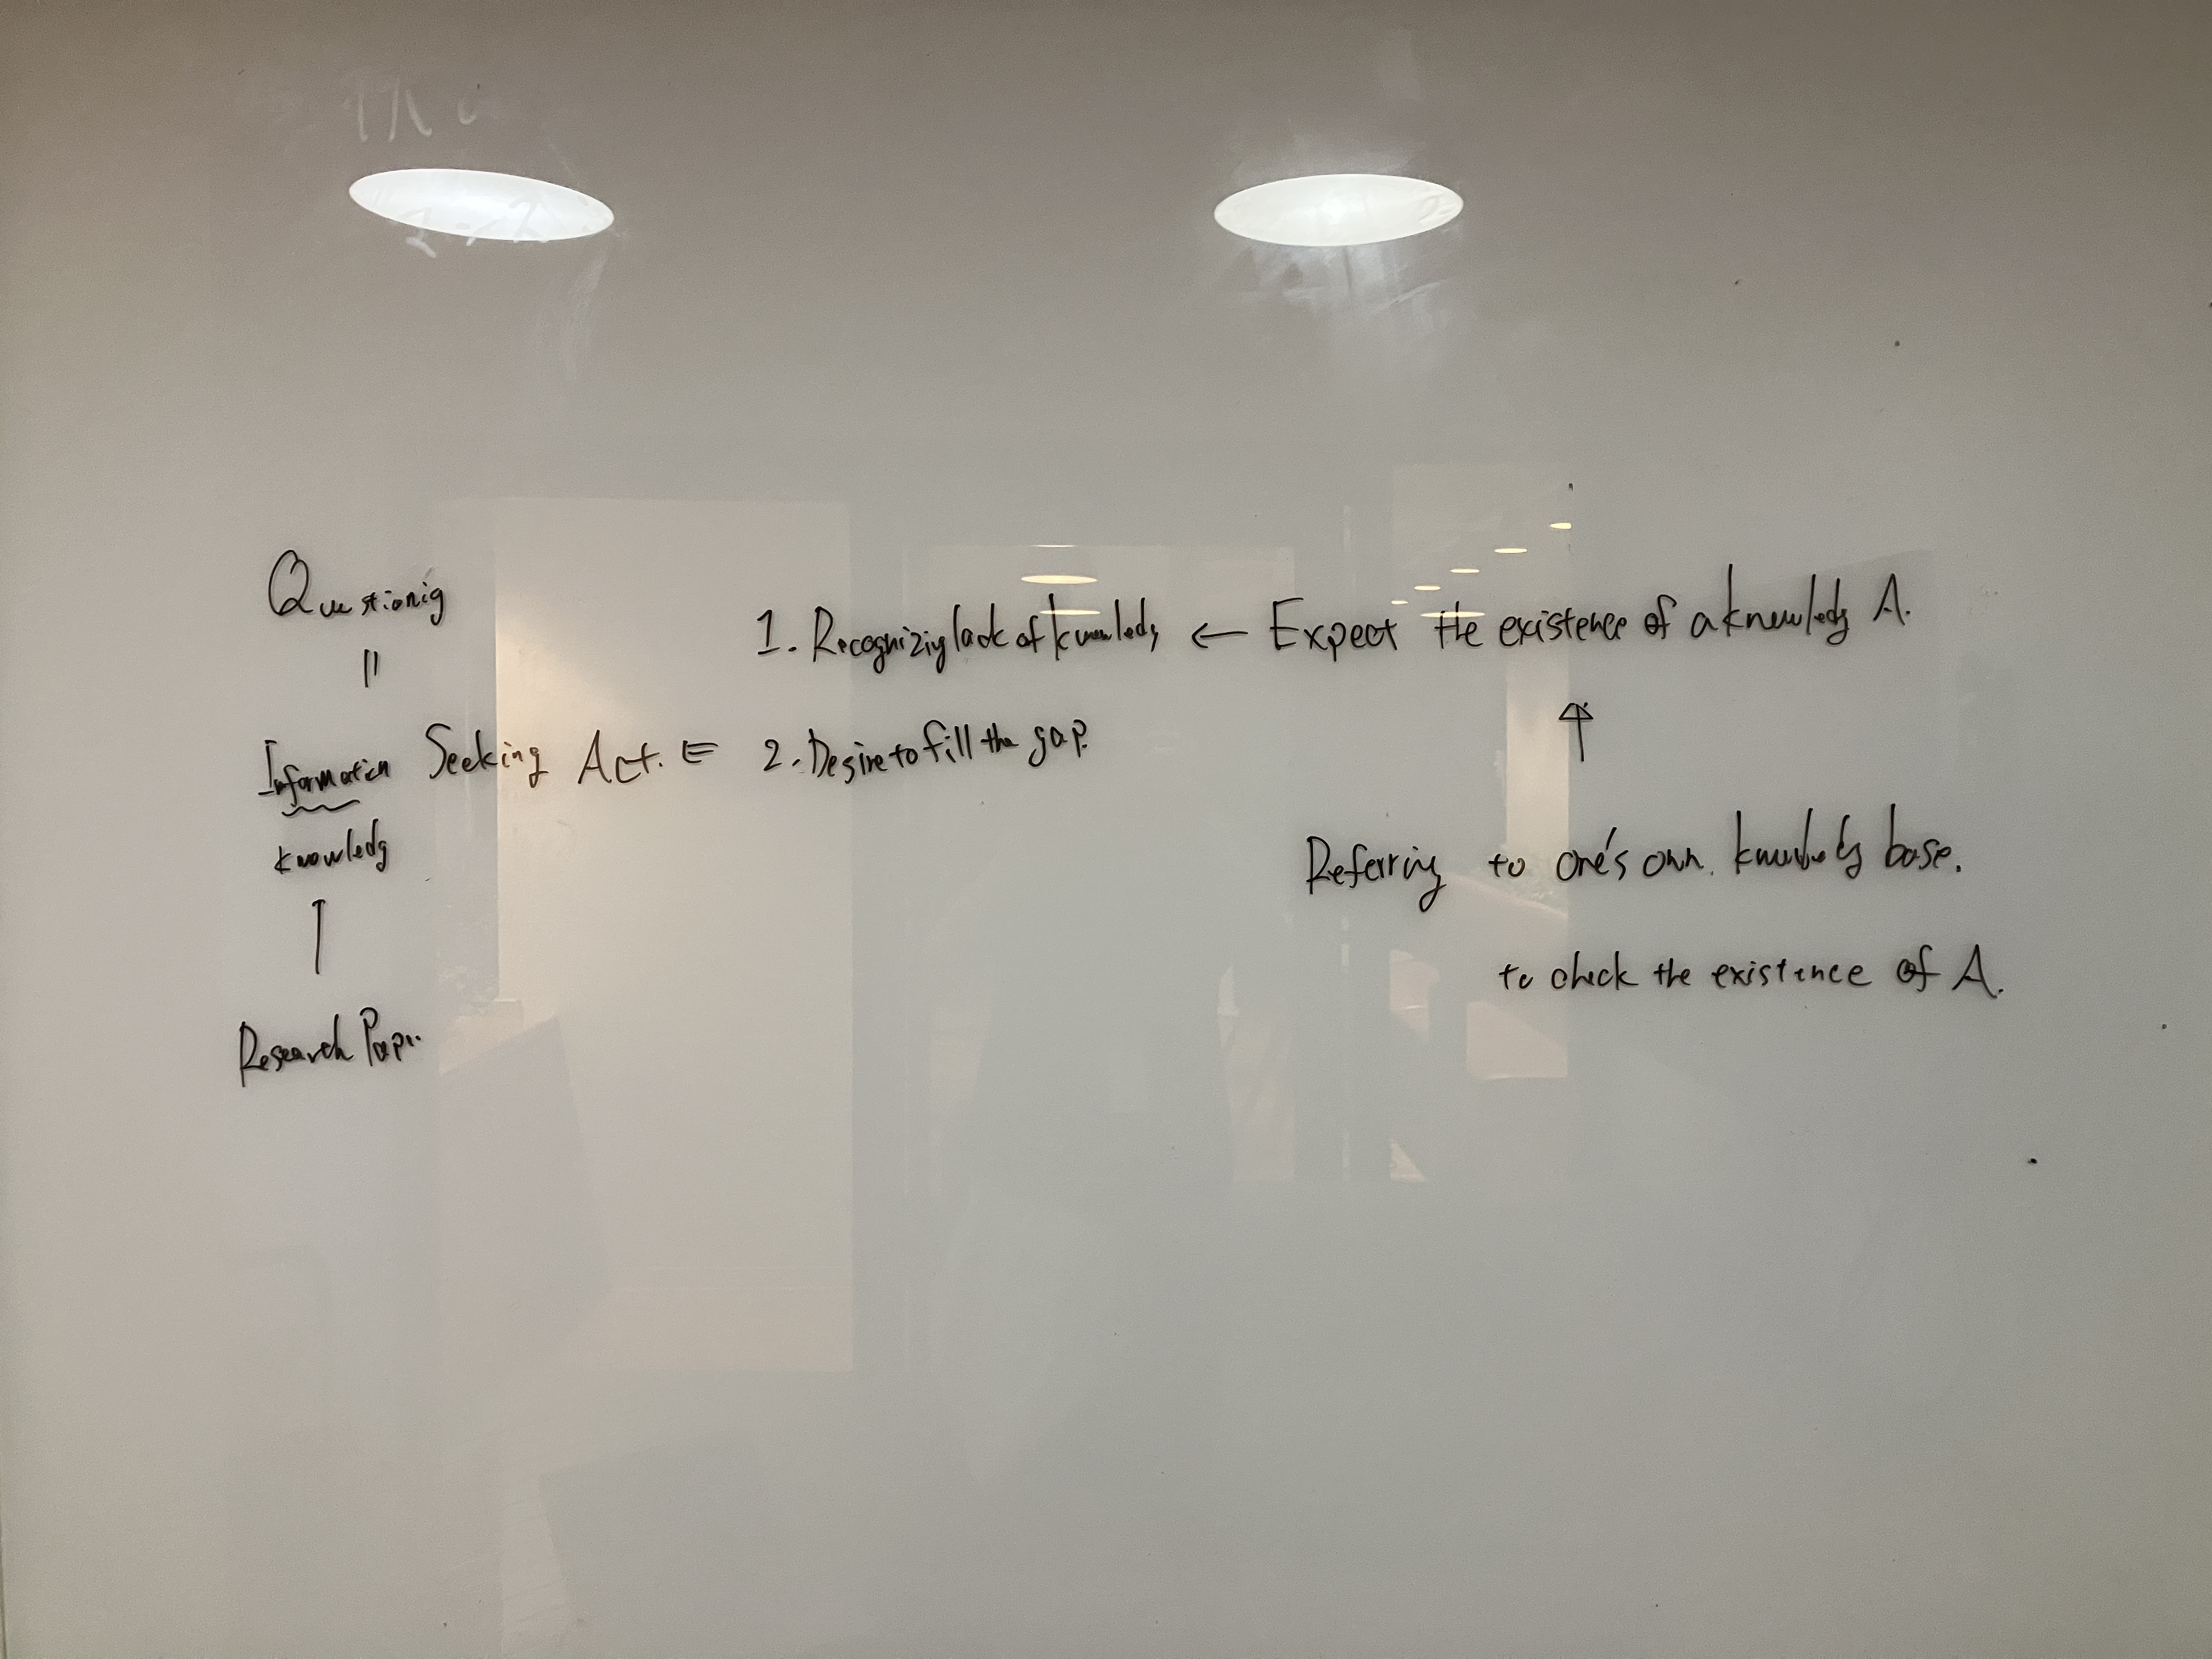
\includegraphics[width=\textwidth]{figs/question_formulation.jpg}
%     \caption{question construction}
%     \label{fig:enter-label}
% \end{figure}

% \subsubsection{How to Identify the Necessary Knowledge for Achieving a Goal?}
% In this situation, we need to consider how to identify the knowledge required to achieve our objectives. Typically, when given a goal, we start by listing the necessary elements to accomplish it. For example, to achieve general artificial intelligence, we may think that it requires the ability to handle language, understand the real world, be proficient in mathematics, and align with human values. To understand the real world, for instance, we may need the capability for interacting with the physical world, processing visual information, and so on. These requirements can be further broken down into multiple necessary elements. By repeating this process, we can narrow down the specific tasks that can be directly addressed. Then, the required knowledge to accomplish those tasks is demanded, and that's where it directly connects to the research question.

% Several things are happening here. Firstly, listing the elements necessary for achieving the goal means generating sub-goals from the main goal. However, it's always a challenging problem to evaluate how a particular sub-goal contributes to the achievement of a given goal. Especially in the case of research, the target might be an too general and ambitious vision that nobody has achieved before, so we need to think about what needs to be done to break it down into appropriate sub-problems. In other words, it is necessary to construct a tree with nodes representing sub-goals.

% Secondly, it is necessary to identify the most important sub-goal from the selected candidate sub-goals. Since only one question can be addressed in the end, it is necessary to select a single sub-goal using some evaluation criteria. This may not be a problem if the sub-goals can be judged on the same evaluation criteria, but in many cases, unrelated sub-goals may arise. For example, to create general artificial intelligence, the development of machine learning theory may be equally important as the advancement of semiconductor technology. However, it may be difficult to compare their importance on the same evaluation axis.

% Thirdly, the question to ultimately arrive at must be verifiable. If the question is not specific, meaningful verification cannot be performed. Overly broad or ambiguous questions can result in countless or trivial answers, or they may be too unclear to provide practical answers. Increasing the specificity of the question corresponds to deepening the depth of the sub-goal tree, so it may be important to construct a sufficiently deep tree and find an efficient way to navigate it. The verifiability is constrained by the knowledge, resources, such as funding and technology, that we currently have. Therefore, when conducting verification in reality, it is necessary to consider such feasibility. Whether to tackle a question with high feasibility or to further divide it into more subtasks for its realization is a matter of judgment. In any case, it is necessary to appropriately evaluate such feasibility. The scope of feasibility is vast, so it is a challenging problem to determine how to consider it in creating intelligent systems.

% Here, we discussed what needs to be done to construct questions that generate the necessary knowledge to achieve the goal. We believe that research that can generate knowledge that is expected to contribute to the achievement of the goal, and that has not been revealed in previous studies, can be considered as ``important'' research. In that sense, it may be important to consider how to achieve the automation of research in this direction.

% In this discussion, we have only touched upon a limited number of points that we personally consider important. However, we believe that there are other important points that should be considered. By seriously reflecting on ``how questions are currently being constructed,'' these points are expected to become clearer.

% Also, in this discussion, we considered the method of outputting questions from the goal through the construction and exploration of a tree structure. However, as mentioned by the predecessors, if an end-to-end approach ultimately becomes a powerful method, it may be more desirable to consider a direction in which questions are directly output from the goal. In particular, even when performing multi-step reasoning, it seems more natural to improve reasoning abilities using the recently developed approaches to multi-step logical reasoning, rather than explicitly considering tree structures. While the development of methods for multi-step reasoning is undoubtedly important in pursuing this direction, this is not a point that needs to be emphasized here as it is being addressed not only in the context of research automation but also more generally. As a discussion focused on the automation of research, it may be worth considering the construction of higher-quality datasets for goals and research questions. For example, it may be possible to construct a dataset by extracting only the ultimate goal and the research questions actually solved from the introductions of papers.

% However, an important point to note here is that the research questions created by humans so far are not necessarily optimal for achieving research goals. Firstly, machines may be capable of maximizing the objective better than humans due to cognitive constraints. Secondly, not all human research has been conducted by working backward from a clear goal. Some studies were conducted simply because they seemed interesting while reading papers. Additionally, as mentioned earlier, abstraction has significantly advanced science, but there are cases where the study of abstraction itself is the

%  objective rather than abstraction in some specific cases. In this regard, simply learning from human data without imitation may constrain the potential capabilities that machines can possess. Therefore, it becomes important to consider how to formulate the maximization of the probability of achieving research goals as a problem, rather than naive learning from human data.

% \subsubsection{How to Search Necessary Knowledge and Recognize the Lack of Knowledge?}
% There are various methods to determine whether the desired knowledge already exists. Typically, it is considered that candidates can be narrowed down in two steps. First, since research papers are composed of questions and their corresponding answers, one can search for papers that have similar questions and answers to the desired knowledge. Once these papers are found, the validity of their verification methods is evaluated. If it is determined that sufficient verification has not been conducted, it can be concluded that the knowledge does not exist.

% In this case, the knowledge itself was considered as the research paper database, so the process involved searching and individually assessing the papers as described above. However, for example, if the knowledge is represented by the distributed representation of a machine itself, the need for the search step may be eliminated. Nevertheless, even in this case, the reliability of the machine's judgment can only be trusted if it has appropriately assessed the effectiveness of its own verification. Therefore, the ability to understand and evaluate verification seems essential in determining the novelty of research.

% \textcolor{red}{TODO: Is question construction information retrieval??}

% \subsubsection{Multiple Reasons for Unknownness}
% new, unimportant, difficult, unnoticed, ... etc.

% \subsubsection{Finding ``Important'' but Unnoticed Questions}

% \subsubsection{Conclusion}
% In summary, the following abilities are required to generate research questions for achieving a specific goal:

% \begin{enumerate}
%     \item Predicting the necessary knowledge from the goal:
%     \begin{enumerate}
%         \item Solving prediction and reasoning problems with long-range relationships.
%         \item Refining knowledge by appropriately incorporating ``good'' qualities such as importance, concreteness, ethics, etc.
%     \end{enumerate}
%     \item Determing the existence of expected knowledge:
%     \begin{enumerate}
%         \item Searching for knowledge directly related to the expected knowledge.
%         \item Determining whether the knowledge has been properly validated.
%     \end{enumerate}
% \end{enumerate}

% 1.a is related to research on improving the reasoning capabilities of machine learning models and on generating intermediate goals in reinforcement learning. If these research fields produce significant results, they can be directly applied. In this sense, it might be beneficial to seek cooperation from those who are actively conducting research in these areas. One of the unique aspects of long-distance inference problems that we think is interesting is the fact that the goal is something that has never been achieved before. This means that you cannot naively learn from data and need to generalize outside of the distribution. Therefore, it's essential to acquire skills not just to recognize patterns but to properly trace the path of reasoning. Moreover, because the goal has not been realized, sub-goals and the paths that connect them are ultimately based on the accumulation of hypothesis generation. In this sense, it can be said that this is a highly uncertain inference. This implies that the choice of which node to select is far from self-evident compared to other logical inference problems. Furthermore, there is the issue of the complexity of the distance between the goal and the question, which is far more intricate than, for example, games or planning everyday trips. For instance, to truly achieve the goal, it may be necessary to build large-scale apparatus like particle accelerators from scratch. This also means that the temporal distance between the goal and the current location is very long. Therefore, it becomes a problem that feedback on how much solving the question contributed to the goal is significantly delayed. While I've only listed a few examples here, there may be other unique challenges and issues that become more serious in research. It will be necessary to work on refining these technical challenges into specific research tasks through discussions with researchers in reasoning and planning.

% 1.b is specific to the automation of research. We first need to be aware that these "good" aspects do not occur naturally. As mentioned before, these are non-epistemic values, so the more autonomy the agent has, the more these must be consciously incorporated. To create an intelligence that constructs ``good'' questions, we first need to understand what we consider a ``good'' question. Also, it's important to turn our attention to things that are not currently considered ``good,'' but should be deemed as ``good'' in essence. Only then can we discuss how to align that value with the agent. Therefore, we think we should start by listing the criteria for determining the ``goodness'' of a question. For this, discussions in the philosophy of science and meta-sciences like the Science of Science may be referenced. Alternatively, large-scale surveys of researchers engaged in actual research could also be important. Once the value is clarified, we might be able to think about creating an intelligence equipped with these values using the value alignment techniques that are currently being developed.

% 2.a is a discussion of Information Retrieval itself. As previously mentioned, research is a process of searching for information from various sources and utilizing it to produce knowledge. Therefore, information retrieval technology is essential, not just for constructing questions. So, it's crucial how much we can get information retrieval researchers involved in this. One of the things strongly related to the automation of research within information retrieval is the search for papers. We will discuss this in the section on information retrieval.

% 2.b is a unique discussion about the automation of research. However, this greatly overlaps with the content to be discussed in the chapter on hypothesis testing. Specifically, what's needed here is the evaluation of testing, whereas what's required for the automation of hypothesis testing is the generation of testing. In this sense, the latter discussion includes the discussion here. Therefore, we will refrain from discussing this here and touch on it later.

% we have listed what we believe are important elements in the construction of questions. However, these are considered important under the assumptions mentioned earlier. For instance, if the goal is not to acquire knowledge necessary for achieving an objective, but to generate knowledge that an individual finds interesting, the necessary elements in question construction (particularly in parts 1.a and 1.b) would change. As previously mentioned, the value of knowledge is determined in relation to context and there's a high degree of uncertainty about how the value of knowledge will evolve in the future. This makes it fundamentally important to have a diverse range of ways to generate questions. The object achievement is highly prevalent and is expected to produce ``important'' knowledge, which is why it is discussed here. However, it is important to discuss what other ways of formulating questions could exist and how they can be implemented.


\subsection{Hypothesis Verification}
verification of hypotheses allows for any action to be considered as long as it is subject to verification, meaning that it updates an individual's beliefs. In this sense, it is believed to be extremely difficult to fully automate the act of verification universally and unconditionally. To achieve complete automation, the realization of physical robots capable of movements at least equivalent to humans in the real world would be necessary, which goes beyond the scope of developing intelligence.

Therefore, to automate this process, it is necessary to proceed with automation gradually, starting from what can be automated. Two directions can be considered as ways to mitigate this problem. The first direction is to break down the verification process and gradually automate parts that are relatively feasible for automation using machine learning. The second direction is to prioritize the automation of research domains where verification is relatively easy. 

\subsubsection{Start from Verification Design}

First, let's explain the former direction. As mentioned earlier, we believe that the verification process can be divided into three stages: formulating a verification plan, preparing for the execution of the verification plan, and executing the verification plan. Among these stages, the execution of the verification plan and the preparation for it require interaction with the physical world in many fields. For example, in certain fields, you may need to purchase and raise rats for training, while in others, you may need to observe physical objects directly. On the other hand, formulating a verification plan is a process that is purely confined to the human mind in a wide range of fields. Of course, in many cases, interacting directly with the physical world can lead to better verification plans, but it is important to note that it is not an absolute requirement. Therefore, to automate the execution and preparation of verification, it is suggested that the power of robotics researchers be leveraged, while machine learning researchers should focus on automating the formulation of verification plans. 

\subsubsection{Narrowing Down the Domain}

Next, let's discuss the second direction, which is to prioritize the automation of verification in research domains where it is relatively easy. As mentioned earlier, the greatest challenge for machine learning researchers in the unified automation of hypothesis verification is the fact that some fields require interaction with the physical world for the execution of verification preparation. Therefore, the second direction is to focus on narrowing down the domains where the execution and preparation of verification take place solely within the computer world and aim for complete automation in these domains.

Many machine learning research and information-related research fall into this domain. However, it remains challenging, but the problem has shifted from reproducing arbitrary movements in physical space to realizing arbitrary operations on a computer, which can be seen as a relaxation of the problem. Research on tool usage using language models that has gained momentum in recent years and research on browser automation are directly related to the automation of this process. If arbitrary operations on a computer can be automated as an extension of these studies, it becomes more realistic for many information-related research fields, fields that can be reduced to pure symbolic operations, and fields where all the resources required for research exist on the web to be fully automated.

From this explanation, it is also clear that in this part of the verification process, which requires execution and preparation, even understanding what verification is may not be necessary as long as the verification plan is perfectly created. The only point at issue is the realization of arbitrary actions within the target space. In other words, as mentioned earlier, these two directions can be pursued in parallel.

Based on the above, we propose that the automation of fields requiring interaction with the physical world be left to capable robotics researchers, and machine learning researchers should initially aim for complete automation of research confined to the computer space. Regarding the autonomy of automating verification plans, it is advisable to first create intelligence that can understand the verification concepts that humans perform. 

Although we can proceed them in parallel, we believe that we should prioritize the automation of verification plan development. This is because, as mentioned repeatedly, the execution and preparation of verification do not require verification-specific capabilities. It aims to acquire more general abilities, and many individuals who are not pursuing research automation are also working towards achieving this. However, the realization of verification plan capabilities is a point of particular interest for those pursuing research automation, and it has not received sufficient attention nor progress unless driven by individuals aiming for research automation. Therefore, we believe that prioritizing the automation in this area would be beneficial.

\subsection{Call for Perspective Papers}

It is necessary to collectively create a perspective paper that includes these automation-related aspects and others. For example, while reading and writing papers are essential skills in research, I am not aware of many recent perspective papers that consider these topics. Furthermore, due to my own lack of knowledge, I do not have a comprehensive understanding of perspective papers on the automation of specific individual studies. I believe many people, not just myself, may be unaware of perspective papers on the automation of research in other fields. Therefore, I suggest creating a space where insights into research automation can be accumulated, and I encourage domain experts to contribute their expertise in areas that may be lacking. This way, I believe the entire endeavor of research automation can accelerate.

\section{How to Approach the Goal}

\subsection{Open Source Projects}

Firstly, I believe that research and development for creating a universal and autonomous artificial researcher should be carried out in an open manner. Furthermore, I think that all research automation projects should strive to share knowledge as much as possible. Firstly, by conducting open research, more people can participate in research automation projects. This leads to an increase in the amount of human resources devoted to the project, enabling faster progress towards achieving the objective. Secondly, sharing knowledge eliminates the need for reinventing the wheel. This reduces wasteful utilization of resources and promotes more efficient progress towards the objective. Thirdly, it removes barriers between individuals sharing the common goal of research automation. Currently, it seems that there is insufficient information sharing between different fields related to the same objective of research automation. For example, research on automating physical property prediction and research on information retrieval from papers seem to exist within different communities. By sharing information, valuable insights that are beneficial to one's own project may be obtained, potentially accelerating the project.

% The ultimate goal is to create an artificial intelligence capable of conducting research autonomously. Therefore, in addition to automating individual modules of research, it is necessary to create a system that can autonomously carry out the entire research process from start to finish. Building such a research process pipeline is one of the sub-goals we aim for.

% This is similar to the pipelines discussed in MLOps in the context of machine learning or scientific workflows mentioned in previous studies. However, unlike those, we envision a system that does not include processing that is heavily dependent on specific research domains or tasks. Instead, we formalize it as a pipeline consisting of modules for question construction, hypothesis generation, and planning and execution of verification, as discussed in Chapter 2. This system autonomously constructs and validates hypotheses for any given question with an unknown answer.


% \section{Others}

